\documentclass[tikz,border=5pt]{standalone}
\usepackage{tikz}
\usetikzlibrary{shapes.geometric, arrows.meta, positioning, shadows}

\begin{document}
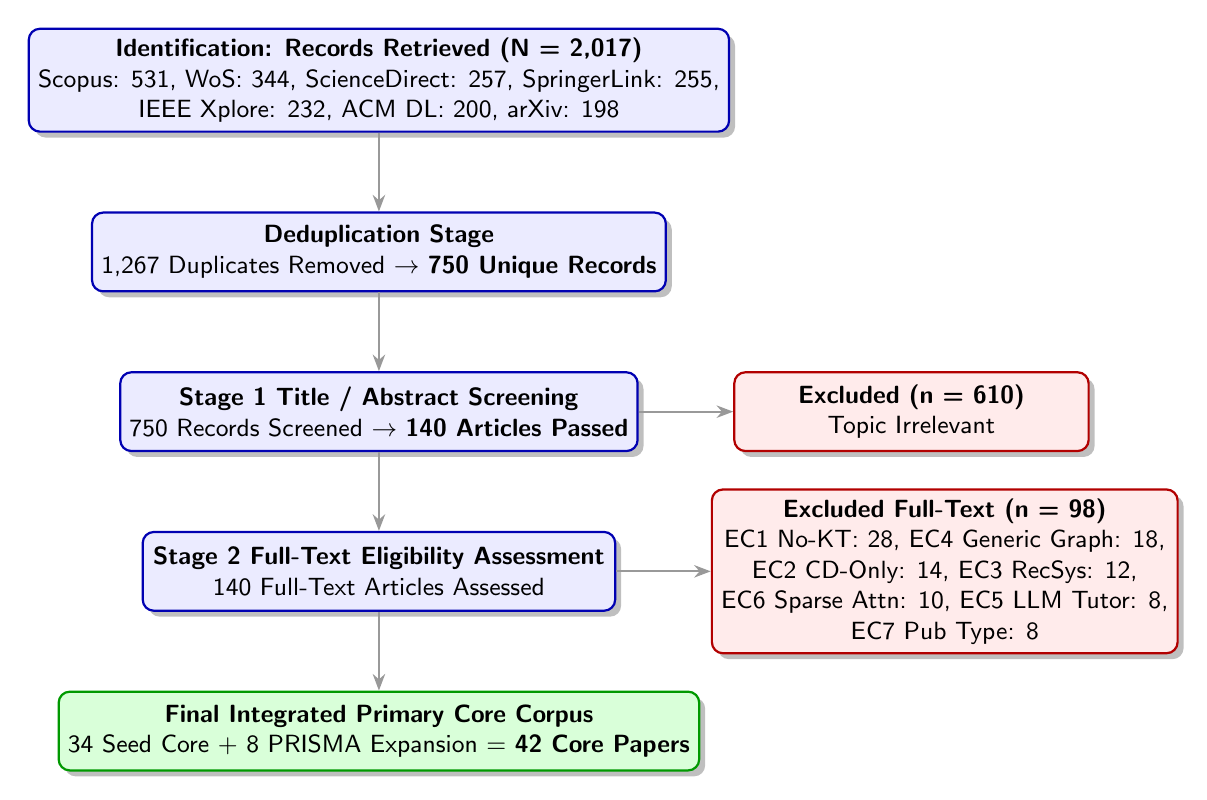
\begin{tikzpicture}[
    node distance=1.2cm,
    font=\sffamily\small,
    stage/.style={rectangle, draw=blue!70!black, fill=blue!8, thick, rounded corners=4pt, align=center, minimum width=6cm, minimum height=1.0cm, drop shadow},
    excl/.style={rectangle, draw=red!70!black, fill=red!8, thick, rounded corners=4pt, align=center, minimum width=4.5cm, minimum height=1.0cm, drop shadow},
    arrow/.style={-{Stealth[length=6pt]}, thick, draw=gray!80}
]

% Nodes
\node[stage] (ident) {\textbf{Identification: Records Retrieved (N = 2,017)}\\Scopus: 531, WoS: 344, ScienceDirect: 257, SpringerLink: 255,\\IEEE Xplore: 232, ACM DL: 200, arXiv: 198};

\node[stage, below=1.0cm of ident] (dedup) {\textbf{Deduplication Stage}\\1,267 Duplicates Removed $\rightarrow$ \textbf{750 Unique Records}};

\node[stage, below=1.0cm of dedup] (screen) {\textbf{Stage 1 Title / Abstract Screening}\\750 Records Screened $\rightarrow$ \textbf{140 Articles Passed}};
\node[excl, right=1.2cm of screen] (excl_screen) {\textbf{Excluded (n = 610)}\\Topic Irrelevant};

\node[stage, below=1.0cm of screen] (fulltext) {\textbf{Stage 2 Full-Text Eligibility Assessment}\\140 Full-Text Articles Assessed};
\node[excl, right=1.2cm of fulltext] (excl_full) {\textbf{Excluded Full-Text (n = 98)}\\EC1 No-KT: 28, EC4 Generic Graph: 18,\\EC2 CD-Only: 14, EC3 RecSys: 12,\\EC6 Sparse Attn: 10, EC5 LLM Tutor: 8,\\EC7 Pub Type: 8};

\node[stage, fill=green!15, draw=green!60!black, below=1.0cm of fulltext] (final) {\textbf{Final Integrated Primary Core Corpus}\\34 Seed Core + 8 PRISMA Expansion = \textbf{42 Core Papers}};

% Arrows
\draw[arrow] (ident) -- (dedup);
\draw[arrow] (dedup) -- (screen);
\draw[arrow] (screen) -- (excl_screen);
\draw[arrow] (screen) -- (fulltext);
\draw[arrow] (fulltext) -- (excl_full);
\draw[arrow] (fulltext) -- (final);

\end{tikzpicture}
\end{document}
